\begin{mdframed}[style=warning]
	\begin{ejercicio}
		La ecuación de movimiento
			$$ m\dot{v} = -mkv, $$
		integrando
			$$ v(t) = v_o e^{-kt}, \qquad \qquad x(t) = \frac{v_o}{k} \qty(1 - e^{-kt}). $$
		Graficando para la velocidad initial $v_o = 10m/s$
		\begin{figure}[H]
			\centering
			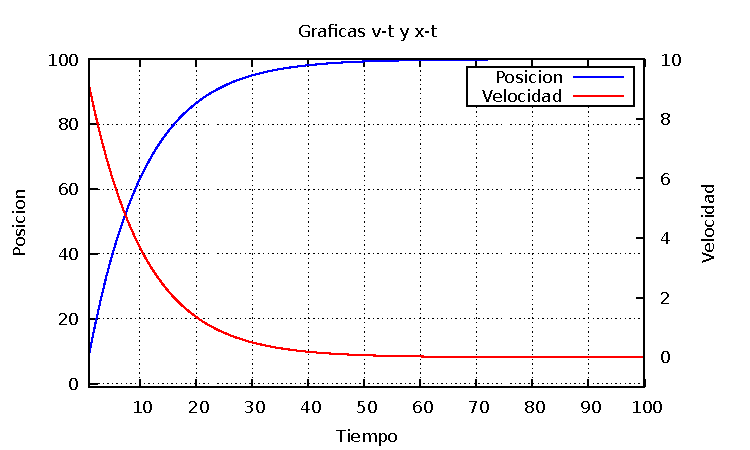
\includegraphics[scale=1]{img/ej1-1.pdf}
			\caption{Grafica Velocidad$-$Tiempo y Posición$-$Tiempo.}
			\label{ej1-1}
		\end{figure}
	\end{ejercicio}
\end{mdframed}

\begin{mdframed}[style=warning]
	\begin{ejercicio}
		Tomando las ecuaciones para cada eje
			$$ x(t) = v_o t\cos{\alpha}, \qquad \qquad y(t) = v_o t \sin{\alpha} - \frac{1}{2} gt^2, $$
		Las coordenadas del punto en la trayectoria cruzada por la línea son $(d\cos{\beta},d\sin{\beta})$. Entonces, calculamos el tiempo para ese punto, dividiendo ambas ecuaciones
			$$ \frac{d\sin{\beta}}{d\cos{\beta}} = \frac{v_o t \sin{\alpha} - \frac{1}{2}gt^2}{v_o t\cos{\alpha}}, $$
		Despejando
			$$ \boxed{t = \frac{2_vo}{g} \qty(\sin{\alpha} - \cos{\alpha} \tan{\beta}).} $$
	\end{ejercicio}
\end{mdframed}

\begin{mdframed}[style=warning]
	\begin{ejercicio}
		Sin resistencia del aire, se tienen que el tiempo para llegar a su altura máxima esta dado por:
			$$ \boxed{t = \frac{v_o}{g}.} $$
		Con resistencia del aire, la ecuación que lo modela es
			$$ m\ddot{y} = -mg - bv, $$
		separando variables e integrando se tiene
			$$ \ln{\abs{\frac{v + \frac{mg}{b}}{v_o + \frac{mg}{b}}}} = -\frac{b}{m} t $$
		como el punto final de la trayectoria es la altura máxima, la velocidad es cero
			$$ t = \frac{m}{b} \ln{\abs{1 + \frac{v_o b}{mg}}}. $$
			
		Expandiendo el logaritmo en series de taylor
			$$ t = \frac{m}{b} \qty(\frac{v_o b}{mg}) \qty[1 - \frac{1}{2} \qty(\frac{v_o b}{mg}) + \frac{1}{3} \qty(\frac{v_o b}{mg})^2 - \cdots] $$
		para un entorno sin resistencia del aire $b \approx 0$
			$$ t = \frac{v_o}{g}. $$ 
	\end{ejercicio}
\end{mdframed}

\begin{mdframed}[style=warning]
	\begin{ejercicio}
		Las ecuaciones para el proyectil son
			$$ \left\{\begin{array}{c}
				x(t) = v_o t \cos{\alpha} \\
				y(t) = v_o t \sin{\alpha} - \frac{1}{2} gt^2 .
			\end{array}\right. $$
		Despejando el tiempo de $x(t)$ y reemplazandolo en $y(t)$; además, tomando $x = D\cos{\beta}$ y $y = D\sin{\beta}$
			$$ D\qty[\frac{gD\cos^2 {\beta}}{2v_o ^2 \cos^2 {\alpha}} - \cos{\beta}\tan{\alpha} + \sin{\beta}] = 0, $$
		luego de un poco de algebra
			$$ \boxed{D = \frac{2v_o ^2 \cos{\alpha} \sin{\alpha - \beta}}{g\cos^2 {\beta}}.} $$
		Derivando respecto a $\alpha$
			$$ \dv{D}{\alpha} = \frac{2v_o ^2}{g\cos^2 {\beta}} \qty[-\sin{\alpha} \sin{\alpha - \beta} + \cos{\alpha} \cos{\alpha - \beta}]\cos{2\alpha - \beta} = 0, $$
		entonces
			$$ \boxed{\alpha = \frac{\pi}{4} + \frac{\beta}{2}.} $$
		El rango máximo es
			$$ \boxed{D_{max} = \frac{v_o ^2}{g(1 + \sin{\beta})}.} $$
	\end{ejercicio}
\end{mdframed}
